\documentclass[11pt,reqno]{amsart}
\usepackage{amsmath}
\usepackage{amssymb}
\usepackage{tikz-cd}
\usepackage[T1]{fontenc}
\usetikzlibrary{automata}
\usetikzlibrary{positioning,arrows}

\begin{document}

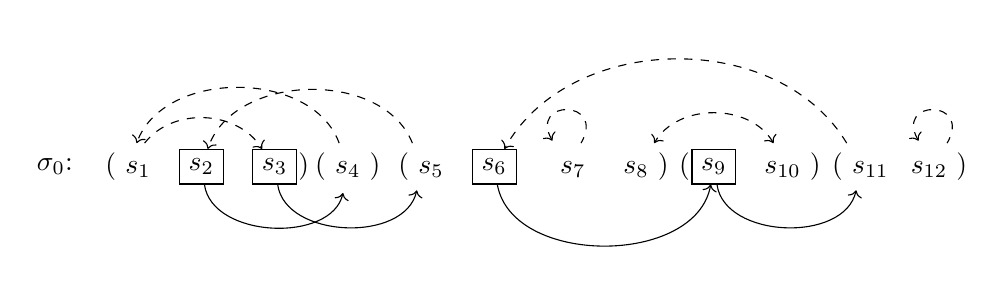
\begin{tikzpicture}[node distance=2cm, scale=0.93]

\node (N) at (-1, 0) {$\sigma_0$:};
\node (1) at (0, 0) {(\,\,$s_1$};
\node[draw] (2) at (1, 0) {$s_2$};
\node[draw] (3) at (2, 0) {$s_3$};
\node (n) at (2.4, 0) {)};
\node (4) at (3, 0) {(\,\,$s_4$\,\,)};
\node (5) at (4, 0) {(\,\,$s_5$};
\node[draw] (6) at (5, 0) {$s_6$};
\node (7) at (6, 0) {{\color{white}(}$s_7$};
\node (8) at (7, 0) {{\color{white}(}$s_8$\,\,)};
\node (nn) at (7.6, 0) {(};
\node[draw] (9) at (8, 0) {$s_9$};
\node (10) at (9, 0) {{\color{white}(}$s_{10}$\,\,)};
\node (11) at (10, 0) {(\,\,$s_{11}$};
\node (12) at (11, 0) {{\color{white}(}$s_{12}$\,\,)};

\draw[->, bend right=80, shorten >=1pt] (2) edge (4);
\draw[->, bend right=80] (6) edge (9);
\draw[->, bend right=80] (9) edge (11);
\draw[->, bend right=80] (3) edge (5);
\draw[->, bend left=55, dashed] (1) edge (3);
\draw[->, bend right=70, dashed] (4) edge (1);
\draw[->, bend right=70, dashed] (5) edge (2);
\draw[->, bend right=60, dashed] (11) edge (6);
\draw[<->, bend right=60, dashed] (10) edge (8);
\draw[<-, dashed,shorten <=1pt] (7) to [out=120,in=60,loop,looseness=4.8] (7);
\draw[<-, dashed,shorten <=1pt] (12) to [out=120,in=60,loop,looseness=4.8] (12);

\end{tikzpicture}

\end{document}